\subsection{Perceptron mutli-couches (MLP)}
\subsubsection*{Neurone}
Tout d'abord focalisons-nous sur le travail d'un neurone.
Sur la Figure \ref{neuronemlp}), $k$ est l'indice du neurone.
\begin{figure}
 \centering
 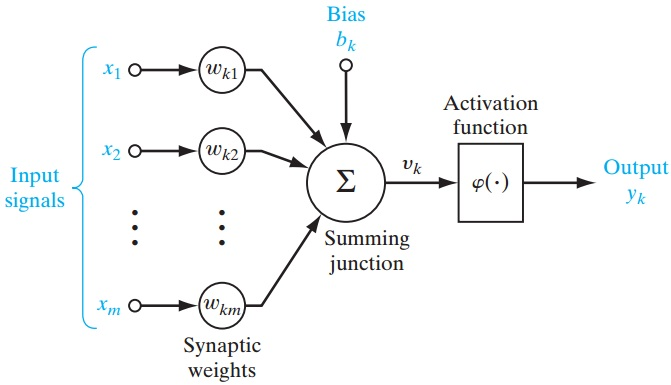
\includegraphics[scale=0.5]{../figures/neurone.jpg}
 \caption{Un neurone artificiel. \textbf{Source}: Haykin\cite{Haykin}}
 \label{neuronemlp}
\end{figure}
Un neurone effectue tout d'abord une somme pondérée de ses entrées \[v_k = b_k+\sum_{j=1}^{m}x_{j}w_{kj}\] où $x$ est le vecteur d'entrée de dimensions $m$.\\
Chaque terme $x_j$ est mutiplié par un poid $w_{kj}$. Ce sont les poids qui seront modifiés lors de la phase d'apprentissage.
Le biai $b_k$ est souvent ajouté à la pondération. Mais pour simplifier les formules, nous pouvons considèrer $b_k$ comme étant l'entrée $x_0 = 1$ de poid fixe $w_{k0} = 1$.
Et la somme pondérée est donc maintenant de la forme \[v_k = \sum_{j=0}^{m}x_{j}w_{kj}\]
Ensuite le neurone applique la \emph{fonction d'activation} $\phi$ sur la somme pondérée.
Le domaine de $y$ est généralement $[0,1]$ ou $[-1,1]$.\cite{Haykin}
La fonction $\phi$ utilisée dépend du problème qu'on veut résoudre (Figure \ref{mlpfonc}).
\begin{figure}
 \centering
 %insert tableau de statistica here
 \textbf{Tableau STATISTICA}
 \caption{Fonctions principalement utilisés dans un neurone d'un MLP. \textbf{Source}: STATISTICA Réseaux de Neurones Automatisés (SANN)\cite{statistica}}
 \label{mlpfonc}
\end{figure}
\subsubsection*{Structure}
\begin{figure}
 \centering
 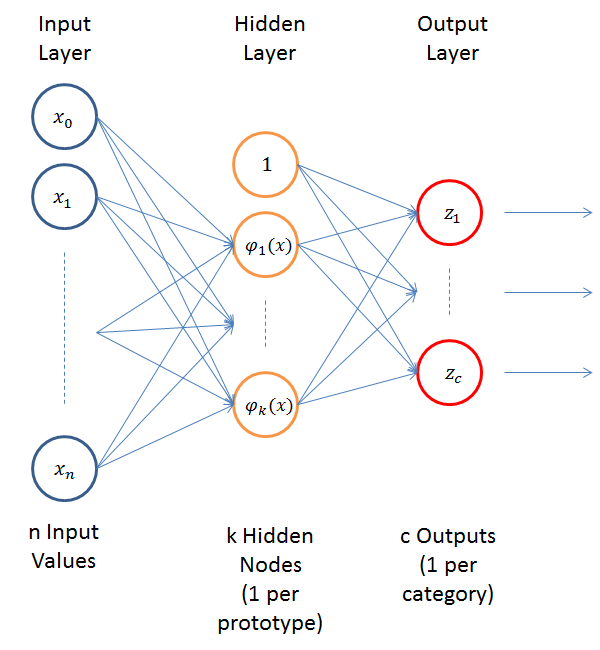
\includegraphics[scale=0.5]{../figures/nnstruct.png}
 \caption{Structure MLP à une couche cachée. \textbf{Source}: McCormick\cite{RBFtuto}}
 \label{structuremlp}
\end{figure}
Un \mlp est composé de plusieurs couches (Figure \ref{structuremlp}):\\
couche d'entrée $\rightarrow$ couches cachées $\rightarrow$ couche de sortie.
Un neurone envoie sa sortie vers tous les neurones de la couche suivante.
Chaque neurones de la couche d'entrée correspond à une dimension du vecteur d'entrée et renvoie juste la valeur de l'entrée dans cette dimension.
Chaque neurones de sortie correspond à une dimension du vecteur de sortie.
Les neurones cachés et neurones de sortie correspondent à la Figure \ref{neuronemlp}.
\subsubsection*{Apprentissage}
Il existe plusieurs algorithmes pour changer les poids sur un réseau. Mais le plus connu pour les \mlp est l'algorithme de de rétropropagation.\cite{Haykin,Gauthier}
Il s'agit d'un algorithme d'\emph{apprentissage supervisé}.
\begin{definition}
L'apprentissage supervisé est une méthode visant à améliorer un approximateur grâce à un calcul d'erreur (appelé aussi mesure de performance\cite{Gauthier}) comparant une sortie générée avec la sortie attendue.
\end{definition}
Nous avons donc besoin d'un ensemble de paires d'entrées/sorties. L'algorithme applique la formule développée ci-dessous pour à tous les neurones sauf les neurones d'entrée.\\

Soit $\phi$, la fonction d'activation. Soit $\phi'$ la dérivée de $\phi$. Soit $Q$ l'\emph{erreur quadratique} utilisé comme mesure de performance.
\[Q = \frac{1}{2}\sum_{i}(a_i-s_i)^2\] où $a_i$ est la sortie du neurone de sortie $i$ et $s_i$ la sortie attendue pour la dimension $i$.
La modification du poid $W_{ij}$ vaut \[\Delta W_{ij} = -\eta\partiel{Q}{W_{ij}}\] où $\eta$ est une constante appelé \emph{pas du gradient}.
Par le théorème de dérivation des fonctions composées, \[\partiel{Q}{W_{ij}} = \partiel{Q}{\phi_i} \partiel{\phi_i}{v_i} \partiel{v_i}{W_{ij}}\]
\begin{thm}[dérivation des fonctions composées]
Soit $f:A~\rightarrow~B : y~\rightarrow~f(y)$ et $g:B~\rightarrow~C : x~\rightarrow~g(x)$. Alors la dérivée de $f~\circ~g$ en $x$ vaut
\[\partiel{f}{x} = \partiel{f}{g} \partiel{g}{x}\]
\end{thm}
Posons $\delta_i = \partiel{Q}{\phi_i} \partiel{\phi_i}{v_i}$. $\delta_i$ est appelé \emph{contridution à l'erreur} du neurone $i$ et est utilisé pour l'apprentissage des neurones de la couche prédédente.
Ensuite, soit $x_i$ l'entrée du neurone $i$,
\begin{equation}
 \begin{split}
  \partiel{v_i}{W_{ij}} & = \partiel{(W_{i0}x_i)}{W_{ij}} + \partiel{(W_{i1}x_i)}{W_{ij}} + ... + \partiel{(W_{ij}x_i)}{W_{ij}} + ... + \partiel{(W_{im}x_m)}{W_{ij}}\\
  ~ & = x_i
  \end{split}
\end{equation}
On a donc \[\Delta W_{ij} = -\eta \delta_i x_i\].
Déterminons la valeur de $\delta_i$.\\

\textbf{Si le neurone $i$ est un neurone de sortie,}
Soit $m$ la dimension de l'entrée $x$ (du neurone). Soit $l$ la dimension du vecteur de sortie du réseau.
\begin{equation}
 \begin{split}
  \partiel{Q}{\phi_i} & = \frac{1}{2} \left( \partiel{(\phi_0 - s_0)^2}{phi_i} + \partiel{(\phi_1 - s_1)^2}{\phi_i} + ... + \partiel{(\phi_i - s_i)^2}{\phi_i} + ... + \partiel{(\phi_l - s_l)^2}{\phi_i} \right)\\
  ~ & = \frac{1}{2}2(\phi_i - s_i)\partiel{(\phi_i - s_i)}{\phi_i}\\
  ~ & = (\phi_i - s_i)\\
  \partiel{\phi_i}{v_i} & = \phi'(v_i)
 \end{split}
\end{equation}
On obtient donc \[\delta_i = (\phi_i - s_i)\phi'(v_i)\]\\

\textbf{Si le neurone $i$ est un neurone caché,}
Soit $m$ la dimension de l'entrée $x$ (du neurone). Soit $n$ le nombre de neurone de la couche suivante.
L'indice $k$ sera utilisé pour désigner un neurone de la couche suivante.
\begin{equation}
 \begin{split}
  \partiel{Q}{\phi_i} & = \sum_{k=1}^{n} \partiel{Q}{\phi_k} \partiel{\phi_k}{v_k} \partiel{v_k}{\phi_i}\\
  ~ & = \delta_k \partiel{v_k}{\phi_i}
 \end{split}
\end{equation}
Or $\phi_i$ est l'entrée du neurone $k$ recevant la sortie du neurone $i$. Posons $W_{ki}$ le poid que $k$ attribue à $\phi_i$.
On obtient donc \[\delta_i = \phi'(v_i) \sum_{k=1}^{n}\delta_{k}W_{ki}\]
\subsubsection*{Applications}
À une couche cachée, un \mlp peut déja servir dans la prédiction de profil.\cite{statistica}\\
Les \mlp sont aussi utilisés en commande de robot par caméra.\cite{Pomerleau}